\begin{document}
\label{appendix_memory_models}
The x86 memory models are a set of six different memory layouts for the x86 CPU operating in real mode, which control how the segment registers are used and the default size of pointers. This appendix summarizes each model.\\

\par
The "Tiny model" is, as you might guess, the smallest of the memory models. All
four segment registers (CS, DS, SS, ES) are set to the same address, so you have a total of 64KiB for all of your code, data, and stack. Near pointers are always used. This model is used for \cw{.com} applications, ensuring backwards compatibility with the CP/M operating system.\\
\vspace{-2pt}
\begin{figure}[H]
\centering
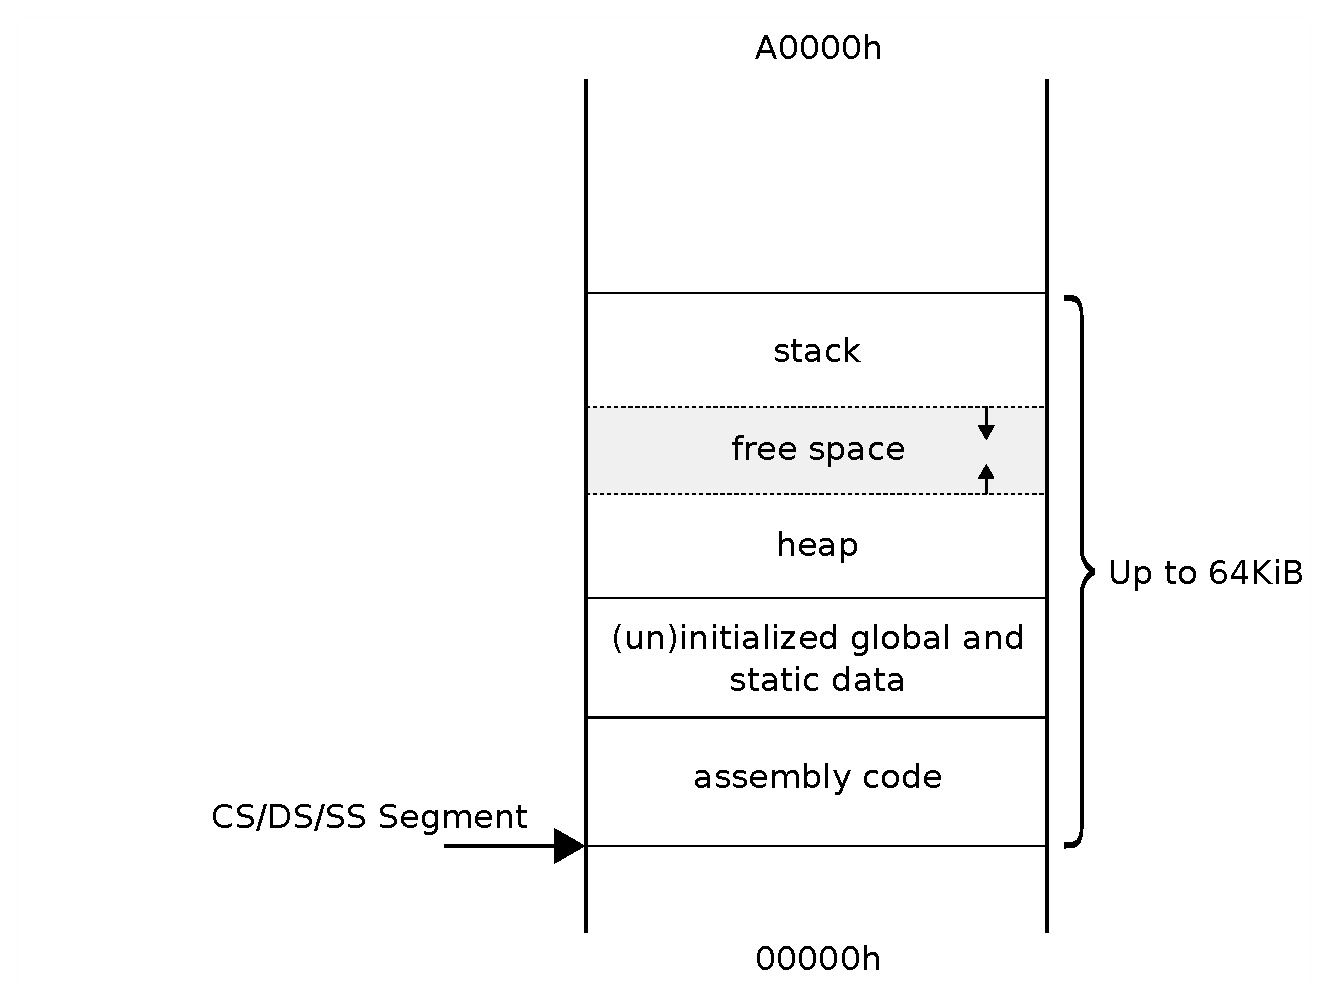
\includegraphics[width=0.65\textwidth]{imgs/drawings/memory/tiny_mm_v2.eps}
\caption{Tiny memory model, total of 64 KiB.}
\label{fig:mm_tiny}
\end{figure}

\pagebreak

The next model is the "small memory model". The code and data segments are different and don't overlap, so you have 64KiB of code and 64KiB of data and stack. Near pointers are
always used. This is a good size for average applications.
\vspace{-2pt}
\begin{figure}[H]
\centering
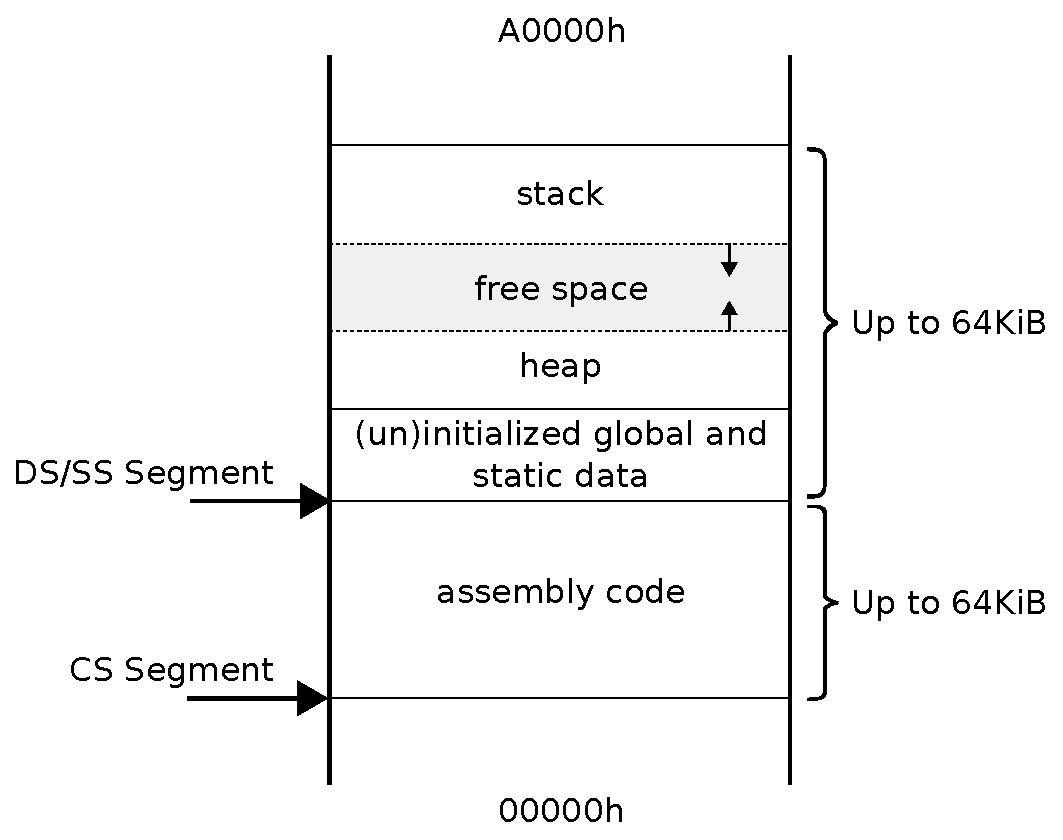
\includegraphics[width=0.65\textwidth]{imgs/drawings/memory/small_mm_v2.eps}
\caption{Small memory model, code and data each have 64KiB.}
\label{fig:mm_small}
\end{figure}

\par
The "medium memory model" is ideal for programs with a large amount of code but minimal data. Far pointers are used for code, but not for data. As a result, data
plus stack are limited to 64K, but code can occupy up to 1 MiB. 
\vspace{-2pt}
\begin{figure}[H]
\centering
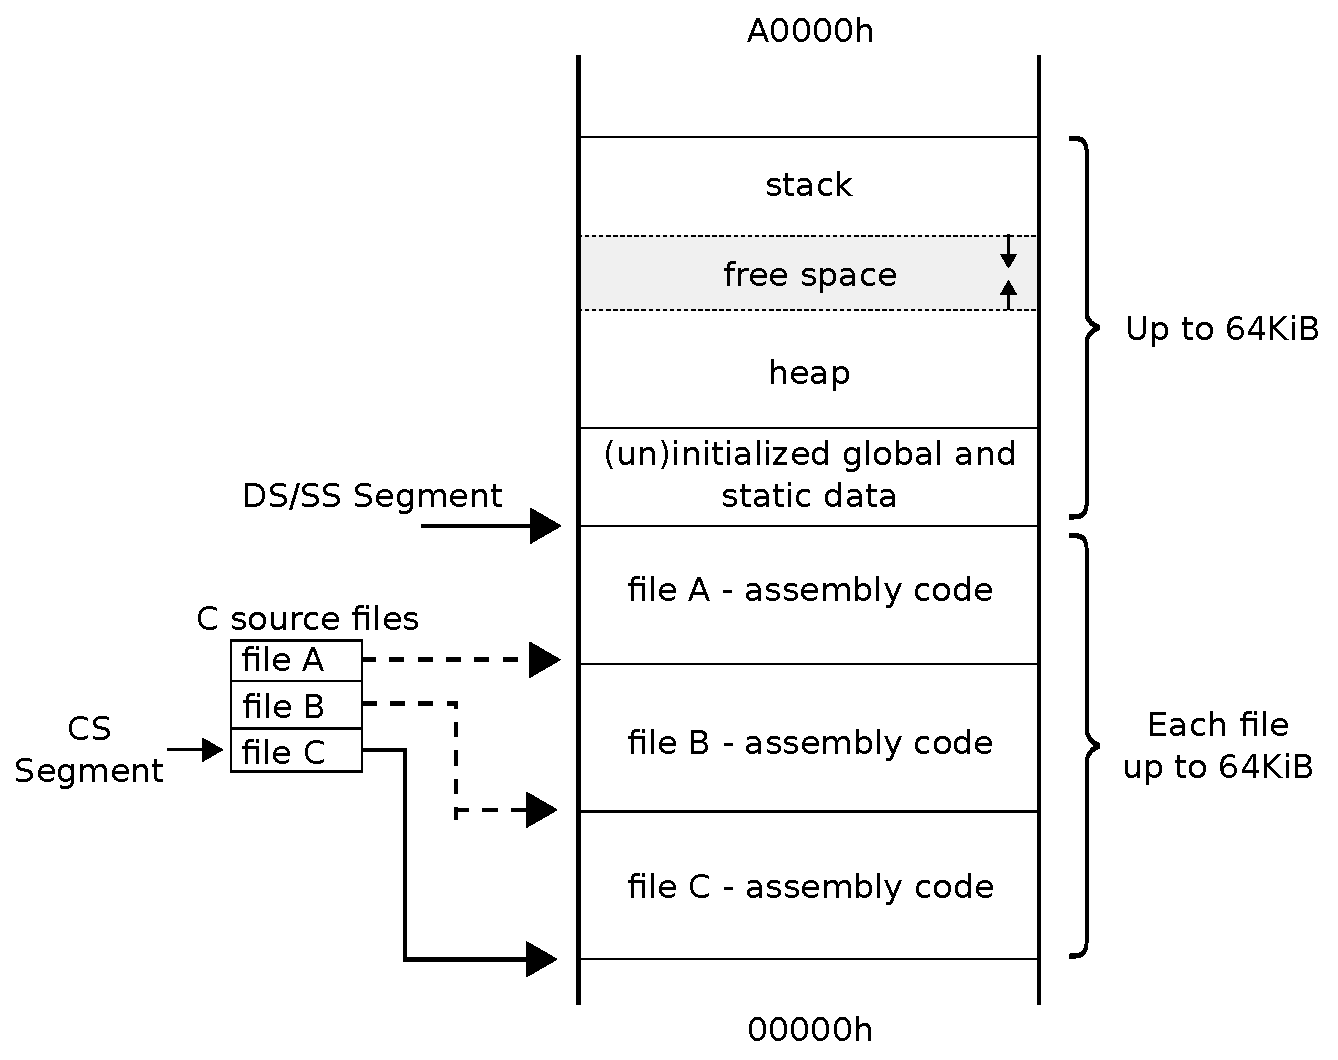
\includegraphics[width=0.65\textwidth]{imgs/drawings/memory/medium_mm_v2.eps}
\caption{Medium memory model, code can be larger than 64KiB.}
\label{fig:mm_medium}
\end{figure}

\par
The opposite of the medium model is the "compact memory model". Here the total function code cannot exceed 64KiB, but there is more space for data. This model is best if code is small but needs to address a lot of data.
\vspace{-2pt}
\begin{figure}[H]
\centering
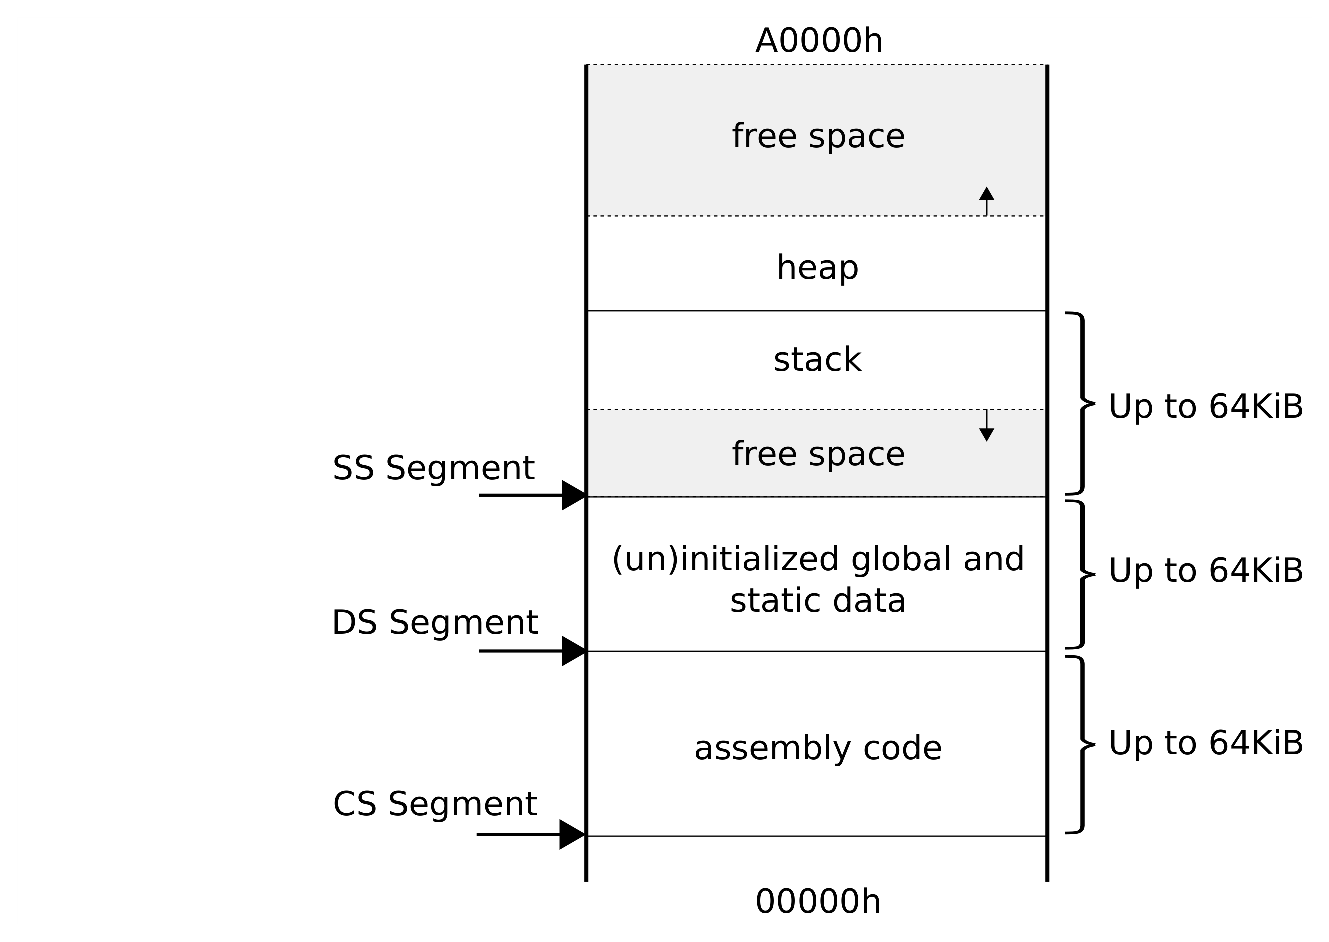
\includegraphics[width=0.65\textwidth]{imgs/drawings/memory/compact_mm_v2.eps}
\caption{Compact memory model, data can be larger than 64KiB.}
\label{fig:mm_compact}
\end{figure}

\vspace{-2pt}
\begin{figure}[H]
\centering
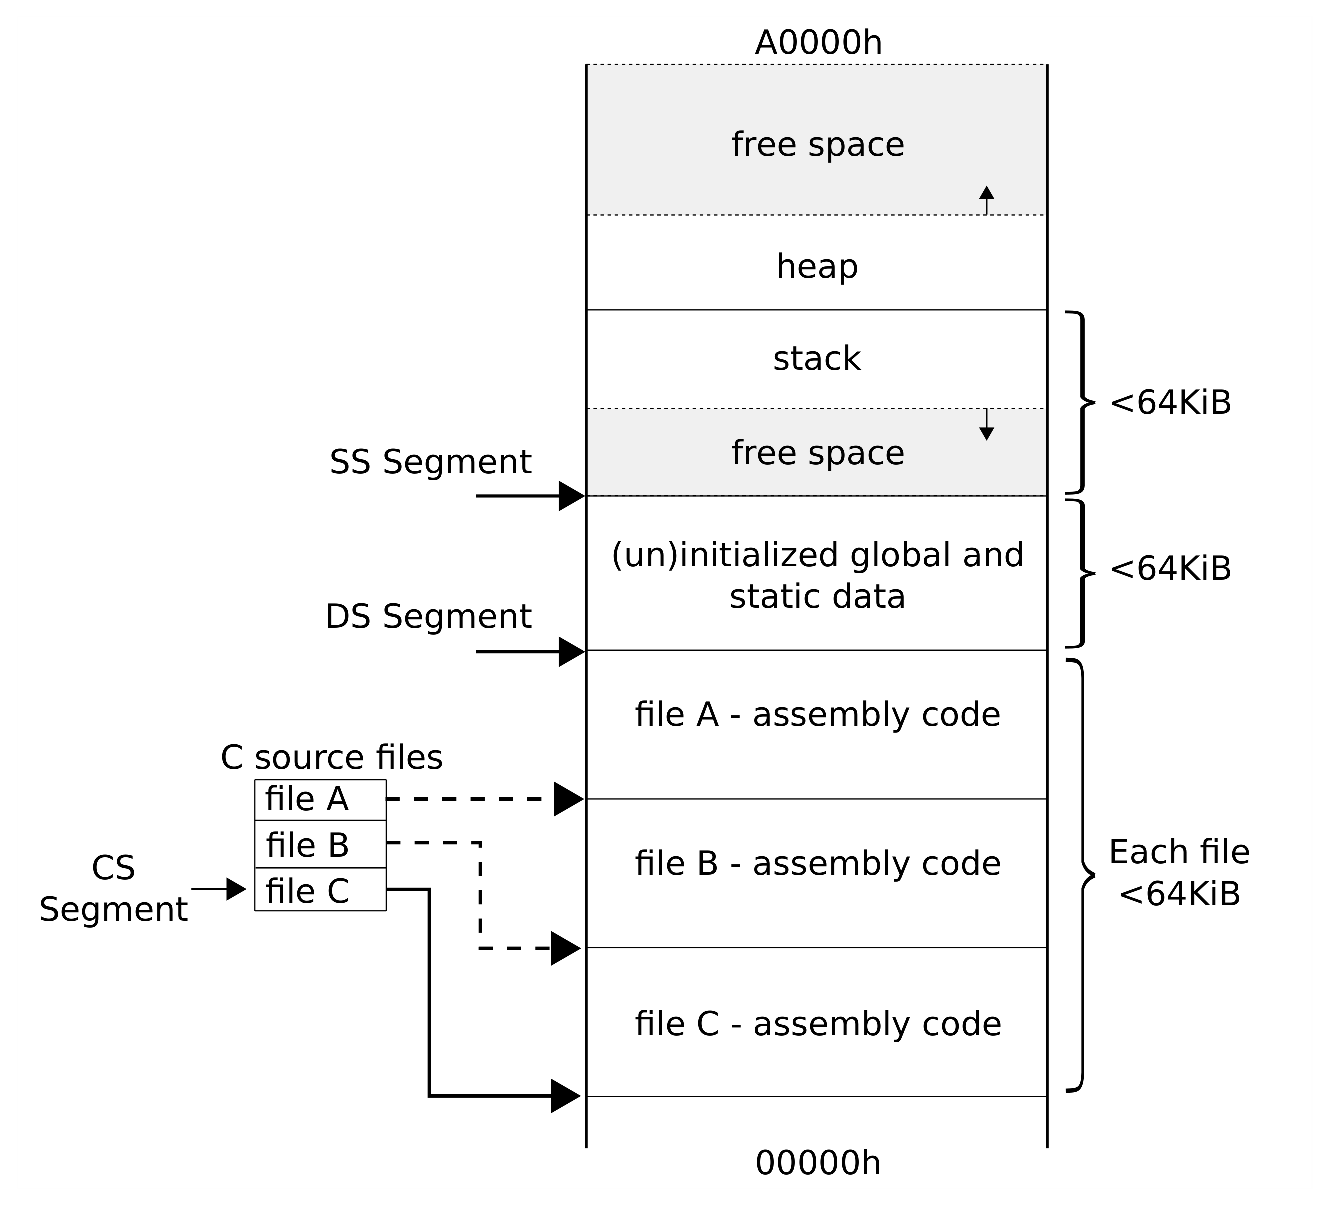
\includegraphics[width=0.65\textwidth]{imgs/drawings/memory/large_mm_v2.eps}
\caption{Large memory model, code and data can be larger than 64KiB.}
\label{fig:mm_large}
\end{figure}



\par
The "large memory model" can deal with function code and data larger than 64KiB. Far pointers are used for both code and data, giving both a 1 MiB range.\\

\par
In all models so far, Borland C++ limits the size of global data to 64KiB. The "huge memory model" sets aside that limit, allowing global data to occupy more than 64KiB using multiple data files. If the source file is too big to fit into one 64KiB data segment, the program must be broken into smaller source files and compiled separately.\\
\begin{figure}[H]
\centering
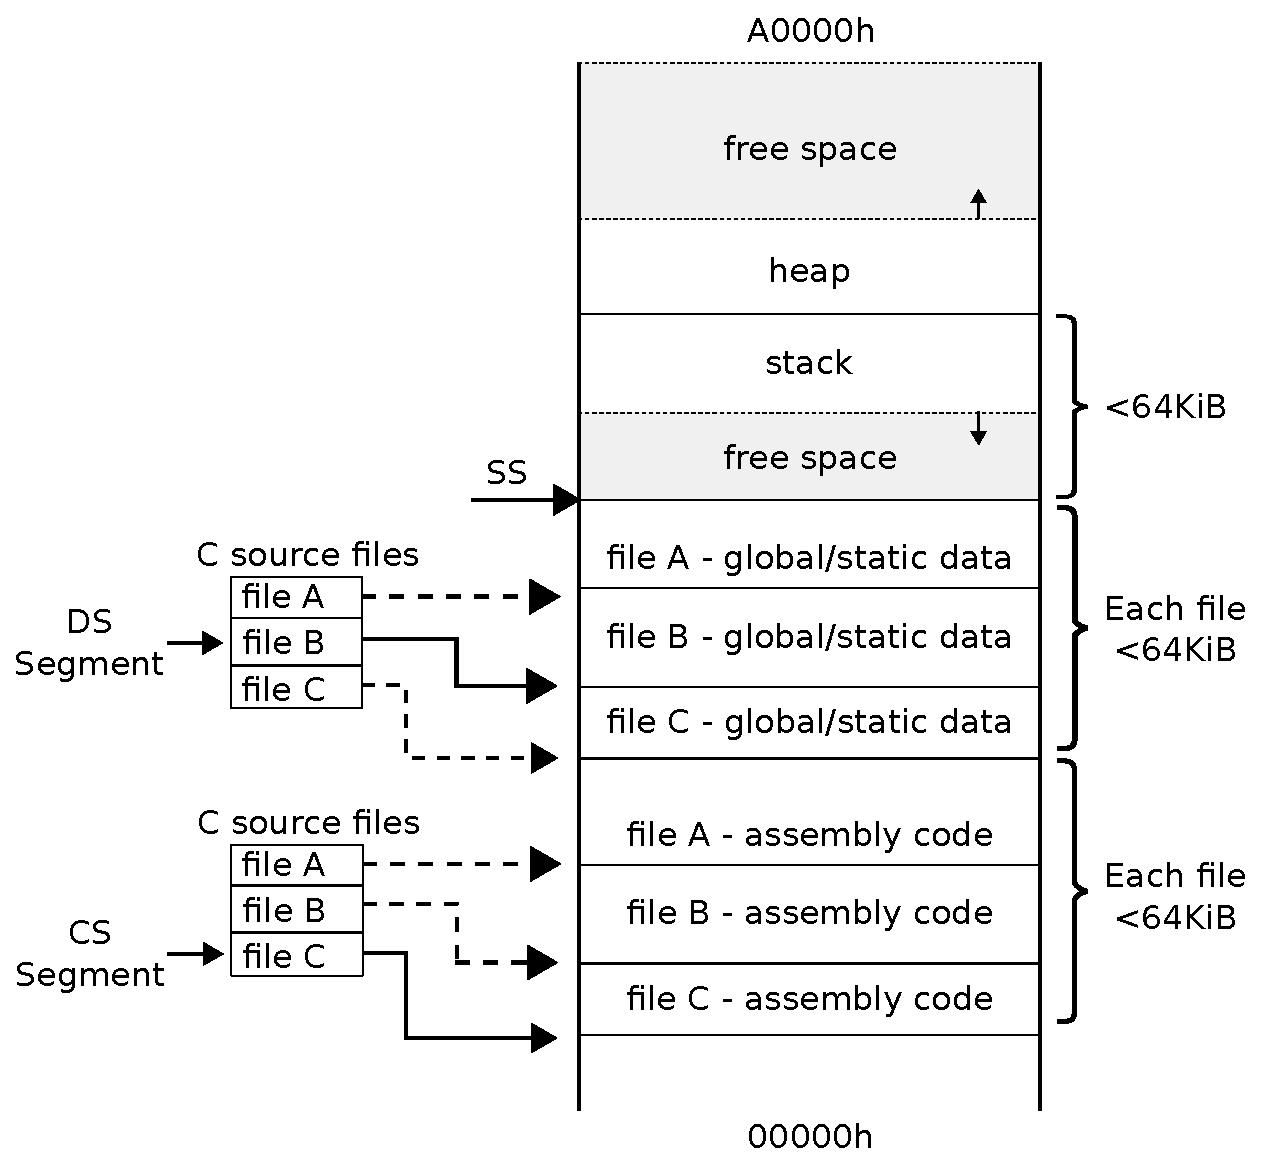
\includegraphics[width=0.68\textwidth]{imgs/drawings/memory/huge_mm.eps}
\caption{Huge memory model, code and global data can be larger than 64KiB.}
\label{fig:mm_large}
\end{figure}

\trivia{Although the name implies differently, the huge memory model in Borland C++ is still limited to segments up to 64KiB using far pointers, and not using huge pointers. The Watcom compiler, which gained popularity in the 90's, was able to break the 64KiB segment barrier using the huge pointer reference for the huge memory model\footnote{See https://open-watcom.github.io/open-watcom-v2-wikidocs/clr.html}.}


\end{document}